%cs-math.tex
\begin{figure}[!t]
\centering
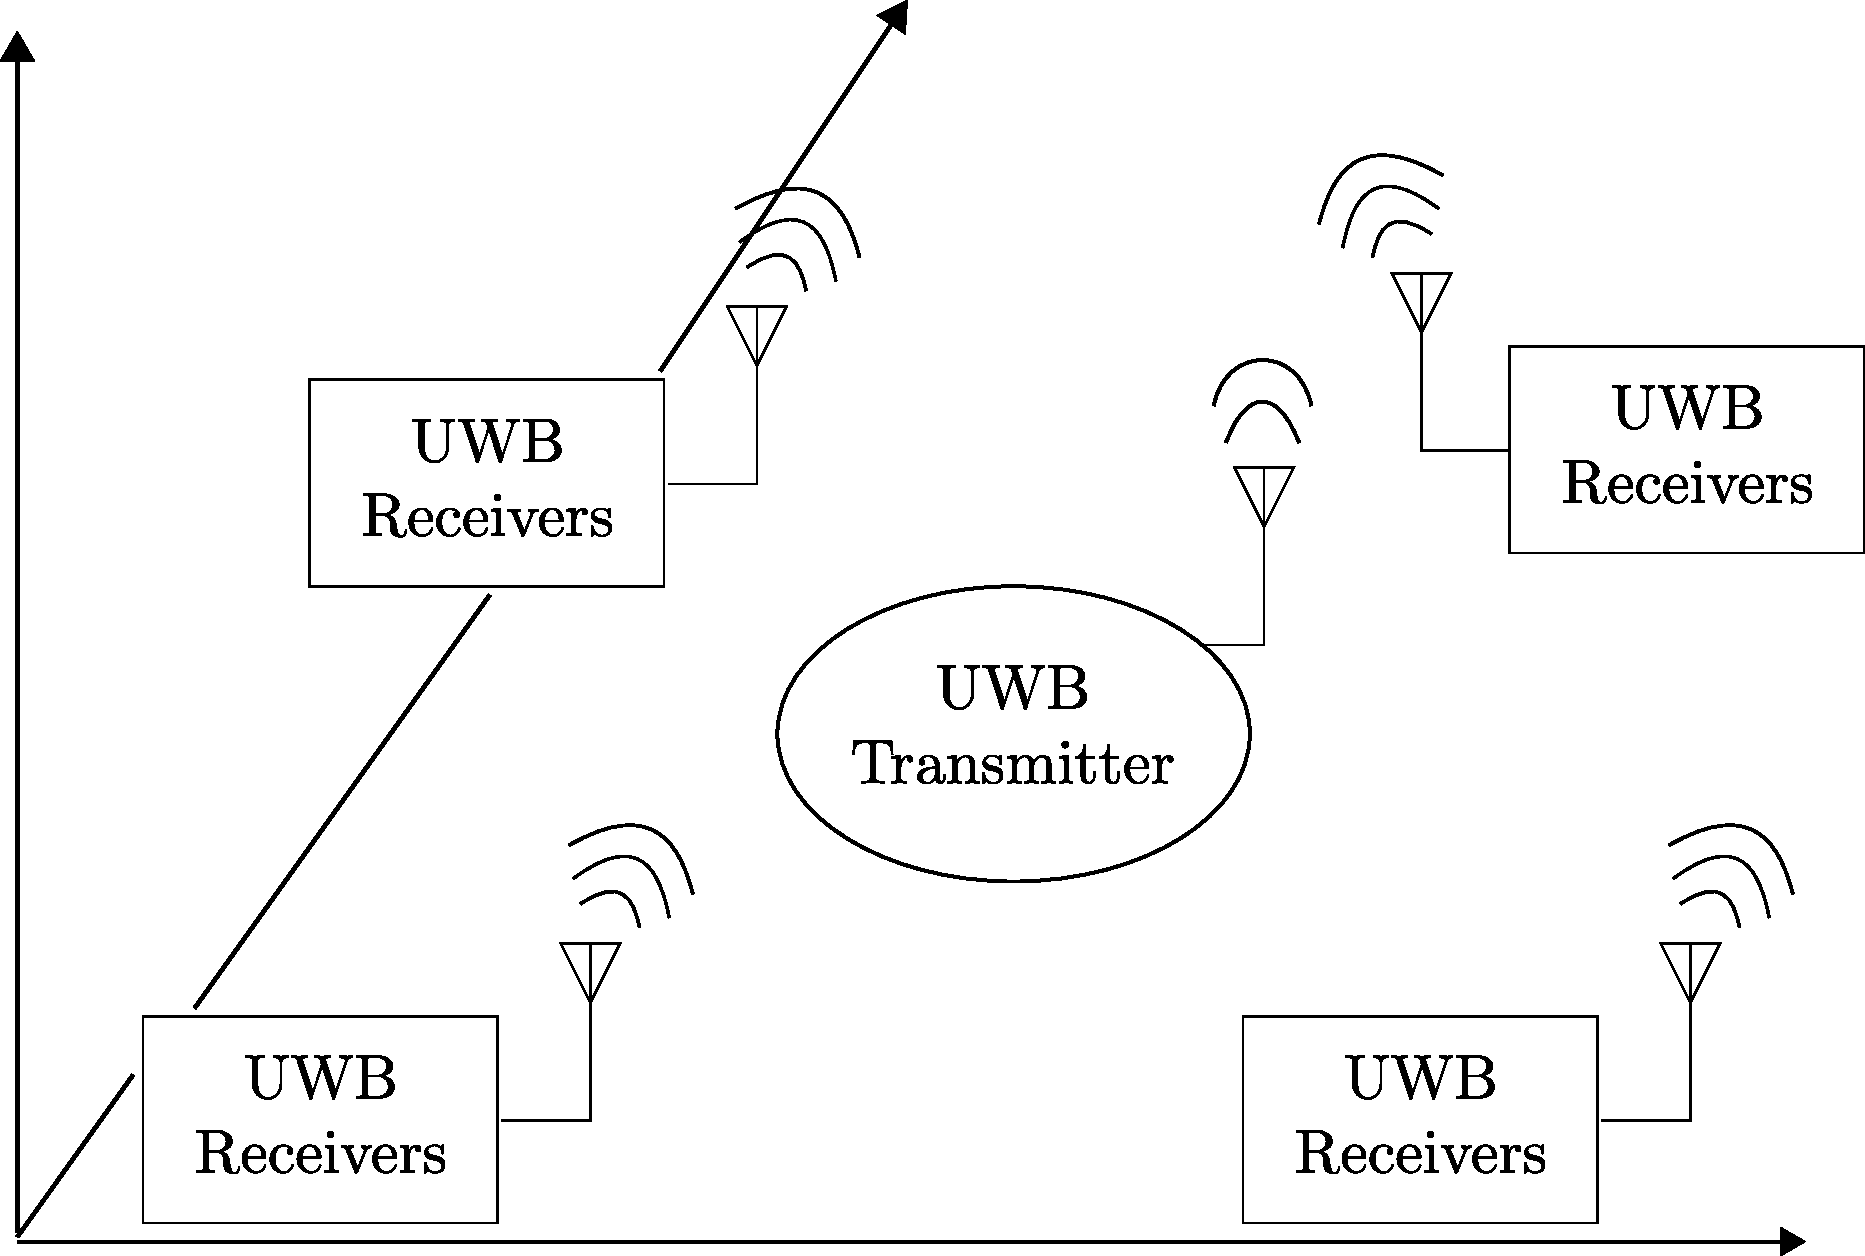
\includegraphics[width=2.7in]{uwb1.pdf}
\DeclareGraphicsExtensions.
\caption{Block diagram of typical UWB indoor communication system}
\label{uwb1}
\end{figure}

Compressed sensing (CS) announces that sparse signals can always be reconstructed from far fewer samples than traditional method of Nyquist Theorem. Consider a task of sampling a signal of $x \in R^N$ using sub-Nyquist rate. Suppose that a group of basis $\Psi$ provides a $K$-sparse representation of signal $x$ as following,  where $k << N$:  
\begin{equation}
\label{eq_sparse}
x=\Psi s=\sum_{l=1}^{K}\psi_l s_l  
\end{equation}
Here $x$ is a linear combination of $K$ basis chosen from $\Psi$, and $s$ is the corresponding coefficients of representing $x$ in the domain constructed by the basis $\Psi$. In CS, $x$  can always successfully be reconstructed from $M$ measurements where $M << N$. The measurements $y$ is generated by projecting $x$ over a matrix $\Phi$ incoherent with $\Psi$, which can be described as $y = \Phi x = \Phi \Psi s$. If the composite matrix $\Phi \Psi$ satisfies restricted isometry property (RIP) \cite{candes2006robust}, then s can be exactly reconstructed by solving the following $l1$-norm minimization problem (\ref{eq_l1_min}):
\begin{equation}
\label{eq_l1_min}
\hat s = \arg\min \| s \|_1 \quad s.t. \quad  y = \Phi \Psi s
\end{equation}
It is shown in \cite{baraniuk2007compressive} that if the composite matrix $\Phi \Psi$ has all random variables taken from a normal distribution, RIP has relatively high probability to be satisfied, indicating that the $l1$-norm minimization (\ref{eq_l1_min}) can provide a stable and robust reconstruction, where only $O(K\ln(N/K))$ sampling points are needed. Therefore, CS provides a novel random sampling paradigm which requires smaller observations and releases the sampling bottleneck defined by Nyquist theory.

Solving this optimization problem (\ref{eq_l1_min}) by linear programming like basis Pursuit (BP) is computationally expensive, but recent greedy algorithms provide alternative solutions that regarded as faster and more efficient, including orthogonal matching pursuit (OMP), compressed sensing matching pursuit(CoSaMP) and iterative hard thresholding (IHT) etc. Among those sparse reconstruction algorithms, CoSaMP and IHT offer the optimal solutions as it works with a minimal number of observations and performs a better recovery robustness to noise, and requires reasonable computational complexities \cite{needell2009cosamp}.

